\section{Tarea}

\subsection{Objetivo}

\begin{itemize}
    \item Implementar un sistema sencillo en Java aplicando los tipos de
    relaciones entre clases y luego dibujar el diagrama UML correspondiente.
    \item Comparar con otros lenguajes de programación: Go, Python,
    JavaScript. (Sólo uno de ellos) Sobre su implementación.
\end{itemize}



\subsection{Problema propuesto: }

\begin{enumerate}[label={ }]
    \item Herencia: Clase Persona (atributos: nombre, edad). Clases hijas: Profesor y Estudiante.
    \item Composición: Clase Curso está compuesta por un Horario (si el curso deja de existir, el horario también).
    \item Agregación: Clase Universidad tiene una lista de Cursos (los cursos pueden existir fuera de la universidad, pero la universidad los ``agrupa'').
    \item Dependencia: Clase Reporte depende del Estudiante porque genera un reporte temporal de sus datos.
\end{enumerate}

Respetar los atributos privados y crear constructores, getters y setters (JavaBeans). Implementar toString() en cada clase.

\begin{enumerate}[label={ }]
    \item Crear un programa principal (Main). 
    \item Se crean 2 profesores y 3 estudiantes. 
    \item Se crean 2 cursos (cada uno con un horario). 
    \item Se agreguen los cursos a la universidad. 
    \item Se genera un reporte de un estudiante.
\end{enumerate}

Dibujar el diagrama UML mostrando las relaciones:




\section{Equipos, materiales y temas utilizados}

\begin{itemize}
    %\item Subsistema de Windows para Linux (WSL) con Ubuntu (versión predeterminada instalada mediante Microsoft Store).
    \item Sistema operativo: Microsoft Windows [Versión 10.0.26100.6584]
    \item MiKTeX-pdfTeX 4.15 (MiKTeX 23.4) \LaTeX.
    \item Strawberry Perl (requerido por MiKTeX para la ejecución de scripts auxiliares en la compilación de ciertos paquetes).
    %\item Helix 25.01.1 (e7ac2fcd)
    \item Visual Studio Code 1.104.0 x64
    \item Git version 2.41.0.windows.1
    \item Cuenta activa en GitHub para la gestión de repositorios remotos.
    \item plantUML
    \item POO.
    \item Lenguaje de programación Java.
    \item Lenguaje de programación JavaScript.
\end{itemize}




\section{URL de Repositorio Github}

\begin{itemize}
    \item URL del Repositorio GitHub para clonar o recuperar.
    \item \url{https://github.com/yhuayhuahi/Teo.git}
    \item URL para el laboratorio (\itemPracticeNumber) en el Repositorio GitHub.
    \item \url{https://github.com/yhuayhuahi/Teo/tree/main/laboratorios/lab\itemPracticeNumber}
\end{itemize}




\section{Desarrollo de las actividades}

\subsection {Actividades}

\subsubsection {Diagrama de clases UML}

Para resolver el problema propuesto se plantea el siguiente diagrama de clases UML:

\begin{figure}[H]
    \centering
    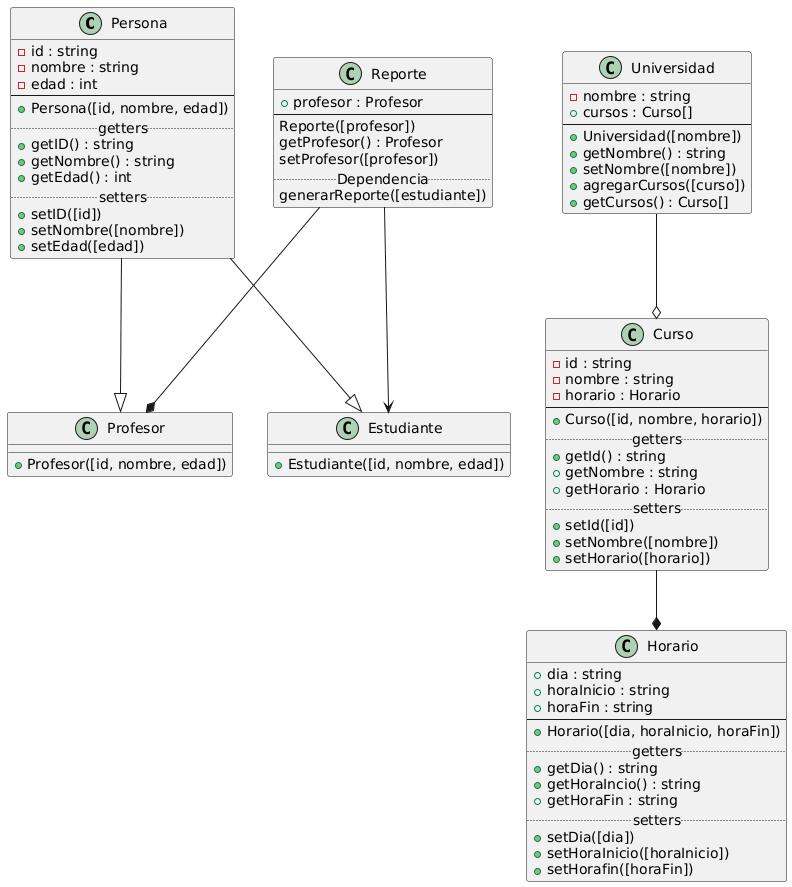
\includegraphics[width=0.8\textwidth]{img/diagrama.png}
    \caption{Diagrama UML de las clases y sus relaciones}
    \label{fig:diagrama_UML}
\end{figure}


\subsubsection {Función Main en Java y JavaScript}

Primero se tiene la funcion Main en Java, en esta se usa todas las clases creadas dentro de la carpeta \textbf{clases}, además se crean 2 profesores, 3 estudiantes, 2 cursos y se genera un reporte de un estudiante.

\begin{lstlisting}[style=java-custom, caption={Función Main en Java}]
    package com.tuorg.poo;
    import com.tuorg.poo.clases.*;

    public class App {
        public static void main(String[] args) {
            System.out.println("=== SISTEMA UNIVERSITARIO ===\n");
            
            // 1. Crear 2 profesores
            Profesor profesor1 = new Profesor("29386481","Dr. Garcia", 45);
            Profesor profesor2 = new Profesor("29386489","Dra. Martinez", 38);

            System.out.println("Profesores creados:");
            System.out.println("- " + profesor1.getNombre() + ", " + profesor1.getEdad() + " años");
            System.out.println("- " + profesor2.getNombre() + ", " + profesor2.getEdad() + " años\n");
            
            // 2. Crear 3 estudiantes
            Estudiante estudiante1 = new Estudiante("12345678","Ana López", 20);
            Estudiante estudiante2 = new Estudiante("87654321","Carlos Ruiz", 22);
            Estudiante estudiante3 = new Estudiante("11223344","María González", 19);

            System.out.println("Estudiantes creados:");
            System.out.println("- " + estudiante1.getNombre() + ", " + estudiante1.getEdad() + " años");
            System.out.println("- " + estudiante2.getNombre() + ", " + estudiante2.getEdad() + " años");
            System.out.println("- " + estudiante3.getNombre() + ", " + estudiante3.getEdad() + " años\n");
            
            // 3. Crear 2 cursos (cada uno con un horario)
            Horario horario1 = new Horario("Lunes", "08:00", "10:00");
            Curso curso1 = new Curso("CS101", "Programación I", horario1);
            
            Horario horario2 = new Horario("Miércoles", "14:00", "16:00");
            Curso curso2 = new Curso("MAT201", "Matemáticas Discretas", horario2);
            
            System.out.println("Cursos creados:");
            System.out.println("- " + curso1.getNombre() + " (" + curso1.getId() + ")");
            System.out.println("  Horario: " + curso1.getHorario().getDia() + " de " + 
                            curso1.getHorario().getHoraInicio() + " a " + curso1.getHorario().getHoraFin());
            System.out.println("- " + curso2.getNombre() + " (" + curso2.getId() + ")");
            System.out.println("  Horario: " + curso2.getHorario().getDia() + " de " + 
                            curso2.getHorario().getHoraInicio() + " a " + curso2.getHorario().getHoraFin() + "\n");
            
            // 4. Crear universidad y agregar los cursos
            Universidad universidad = new Universidad("Universidad Tecnológica Nacional");
            universidad.agregarCursos(curso1);
            universidad.agregarCursos(curso2);
            
            System.out.println("Universidad: " + universidad.getNombre());
            System.out.println("Cursos agregados a la universidad:");
            for (Curso curso : universidad.getCursos()) {
                System.out.println("- " + curso.getNombre() + " (" + curso.getId() + ")");
            }
            System.out.println();
            
            // 5. Generar un reporte de un estudiante
            Reporte reporte = new Reporte(profesor1);
            System.out.println("=== GENERACIÓN DE REPORTE ===");
            reporte.generarReporte(estudiante1);
            
            // Generar otro reporte para mostrar más funcionalidad
            Reporte reporte2 = new Reporte(profesor2);
            reporte2.generarReporte(estudiante2);
            
            System.out.println("\n=== FIN DEL PROGRAMA ===");
        }
    }
\end{lstlisting}

Ahora se tiene la funcion Main en JavaScript, en esta se usa todas las clases creadas dentro de la carpeta \textbf{clases}, además se crean 2 profesores, 3 estudiantes, 2 cursos y se genera un reporte de un estudiante.

\lstinputlisting[style=javascript-style, caption={Función Main en JavaScript}]{../l-javascript/index.js}


\subsubsection{Pruebas de ejecución:}

\begin{itemize}
    \item Se verificó la creación de los objetos de las clases \texttt{Profesor}, \texttt{Estudiante}, \texttt{Curso} y \texttt{Universidad}.
    \item Se comprobó que los reportes generados mostraran la información correcta de los estudiantes.
    \item Se validó que los horarios de los cursos se establecieran correctamente.
\end{itemize}

\textbf{Ejecución en Java:}

\begin{figure}[H]
    \centering
    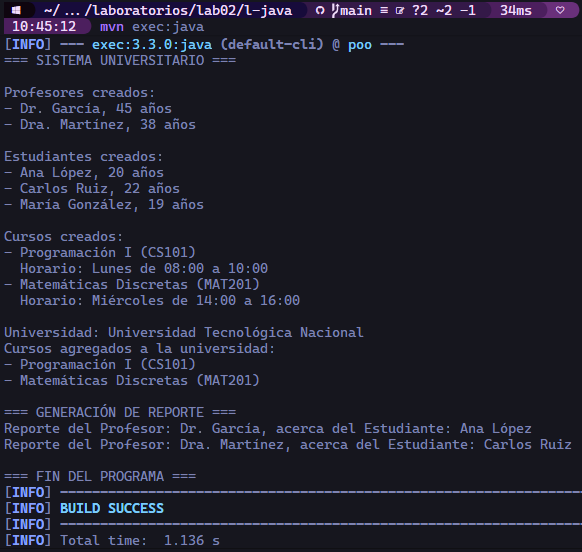
\includegraphics[width=0.8\textwidth]{img/prueba_ejecucion_java.png}
    \caption{Ejecución del programa en Java}
    \label{fig:ejecucion_java}
\end{figure}

\textbf{Ejecución en JavaScript:}

\begin{figure}[H]
    \centering
    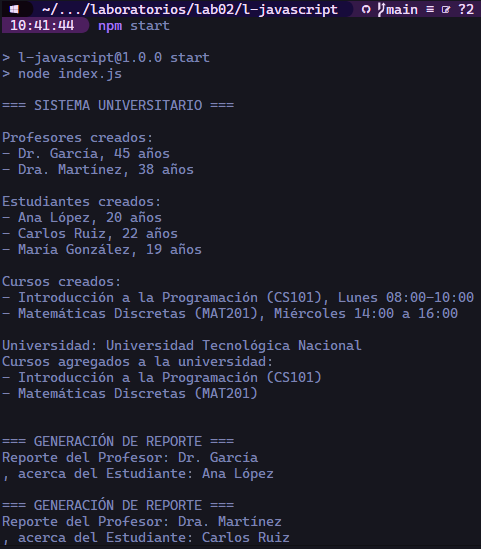
\includegraphics[width=0.8\textwidth]{img/prueba_ejecucion_javascript.png}
    \caption{Ejecución del programa en JavaScript}
    \label{fig:ejecucion_javascript}
\end{figure}



\subsection {Commits realizados}

\subsubsection {Primer Commit}

\begin{itemize}
    \item Este commit se realizo despues de inciar un mini-projyecto en java usando maven como herramienta.
    \item Se crearon las clases requeridas representadas en el diagrama de clases UML, elaborado en PlantUML.
    \item Una clase main para probar el funcionamiento de las clases implementadas.
\end{itemize}

\begin{figure}[H]
    \centering
    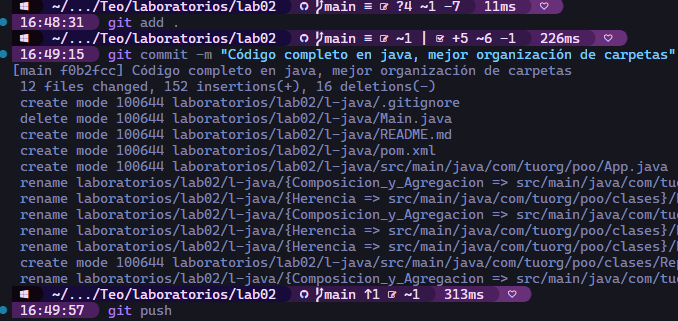
\includegraphics[width=0.8\textwidth]{img/commit01.png}
    \caption{Primer commit}
\end{figure}


\subsubsection {Segundo Commit}

\begin{itemize}
    \item Este commit se hizo despues de modificar el acceso de alguna propiedades de las clases a private.
    \item Antes de este commit, todas las propiedades eran publicas.
\end{itemize}

\begin{figure}[H]
    \centering
    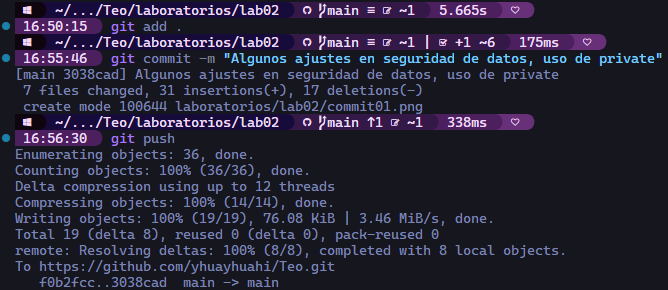
\includegraphics[width=0.8\textwidth]{img/commit02.png}
    \caption{Segundo commit}
\end{figure}


\subsubsection {Tercer Commit}

\begin{itemize}
    \item Este commit se hizo despues de replicar el código de Java a JavaScript.
    \item Se creo una carpeta llamada l-javascript y se implemento todo el código en este lenguaje.
    \item Se verificó que el código en JavaScript funcione correctamente.
\end{itemize}

\begin{figure}[H]
    \centering
    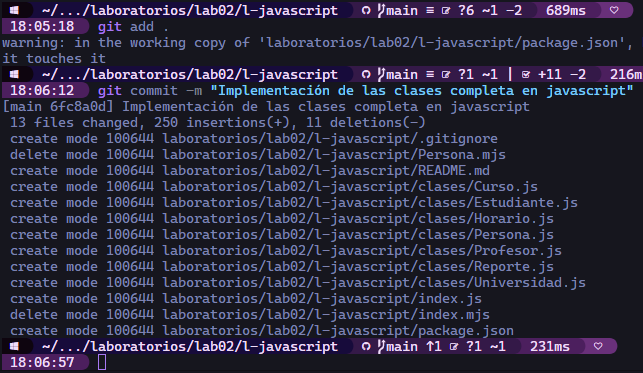
\includegraphics[width=0.8\textwidth]{img/commit03.png}
    \caption{Tercer commit}
\end{figure}


\subsubsection {Cuarto Commit}

\begin{itemize}
    \item Este commit se hizo despues de agregar el método toString() en cada clase.
    \item Este método permite representar el objeto como una cadena de texto
\end{itemize}

\begin{figure}[H]
    \centering
    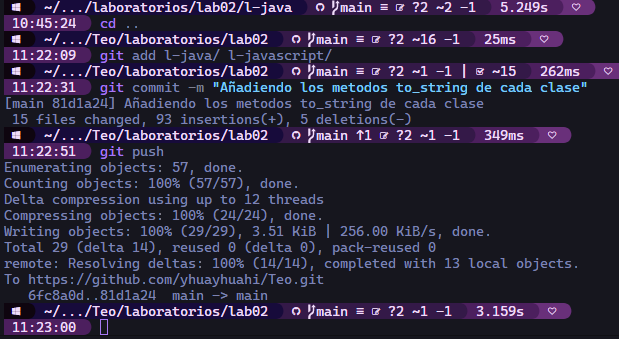
\includegraphics[width=0.8\textwidth]{img/commit04.png}
    \caption{Cuarto commit}
\end{figure}

\subsection {Estructura del laboratorio}

A continuación se muestra la estructura de archivos y carpetas del laboratorio realizado:
Claramente los archivos de compilación de Java y otros que se pudieron generar no se subieron al repositorio.

\begin{figure}[H]
    \centering
    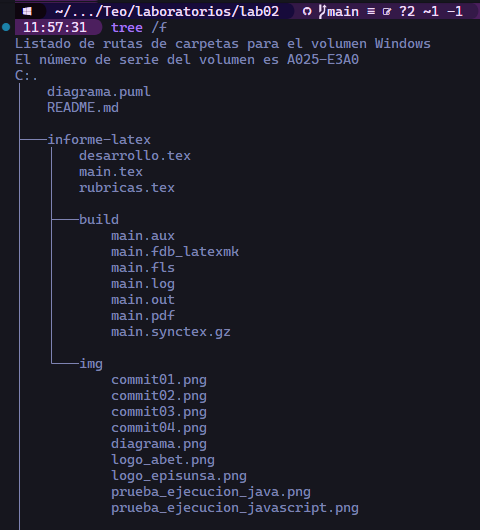
\includegraphics[width=0.8\textwidth]{img/estructura01.png}
\end{figure}

\begin{figure}[H]
    \centering
    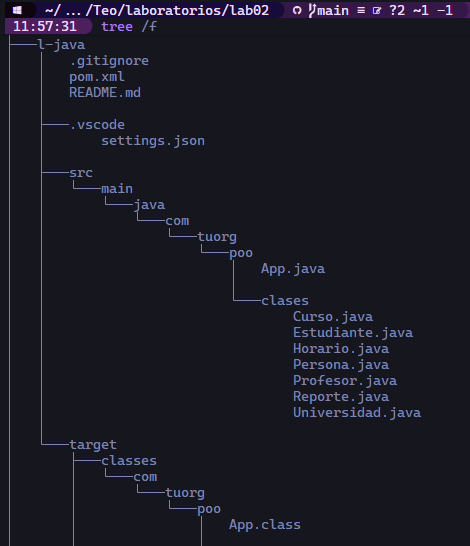
\includegraphics[width=0.8\textwidth]{img/estructura02.png}
\end{figure}

\begin{figure}[H]
    \centering
    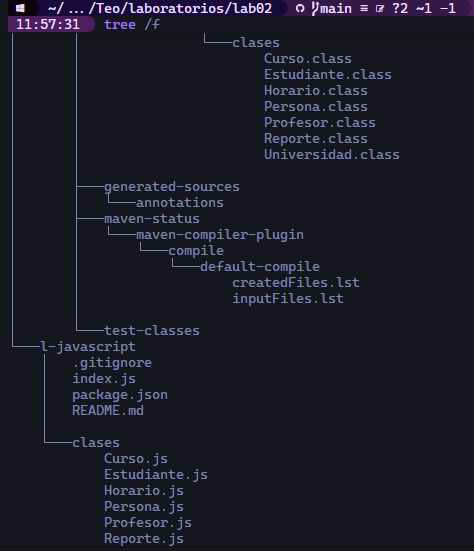
\includegraphics[width=0.8\textwidth]{img/estructura03.png}
\end{figure}




\section{Cuestionario}

\subsection{¿Qué diferencias puede resaltar en las implementaciones de los dos lenguajes de programación en POO?}

\begin{itemize}
    \item \textbf{Sintaxis:} Java tiene una sintaxis más estricta y verbosa, mientras que JavaScript es más flexible y concisa.
    \item \textbf{Tipado:} Java es un lenguaje de tipado estático. JavaScript es un lenguaje de tipado dinámico.
    \item \textbf{Clases y Prototipos:} Java utiliza clases para definir objetos y herencia, mientras que JavaScript utiliza prototipos. Aunque ES6 introdujo la sintaxis de clases en JavaScript, internamente sigue utilizando prototipos.
    \item \textbf{Encapsulamiento:} En Java, el encapsulamiento se logra mediante modificadores de acceso (private, protected, public). En JavaScript, el encapsulamiento se puede lograr utilizando closures o la nueva sintaxis de campos privados (con el prefijo #).
    \item \textbf{Herencia:} Java utiliza herencia basada en clases, mientras que JavaScript utiliza herencia basada en prototipos. Esto afecta cómo se crean y extienden los objetos.
\end{itemize}


\subsection{¿En su implementación dónde se puede evidenciar la protección de datos o la seguridad utilizando la técnica de la programación orientada a objetos?}

Sí, en la implementación de las clases se puede evidenciar la protección de datos a través del uso de modificadores de acceso como private y protected. Esto permite que ciertas propiedades y métodos sean inaccesibles desde fuera de la clase, lo que ayuda a mantener la integridad del objeto y a prevenir modificaciones no autorizadas. Además, el uso de métodos getter y setter proporciona un control adicional sobre cómo se accede y modifica el estado interno de un objeto.




